% based on poster for ASE 2009 by Martin Weiglhofer

\documentclass[final,hyperref={pdfpagelabels=false}]{beamer}
\setbeamertemplate{caption}[numbered]
\mode<presentation>{\usetheme{TUGraz}}

\usepackage{CJKutf8}
\usepackage{amsmath,amsthm,amssymb,latexsym}
\usepackage{graphicx}
\usepackage{multirow}
\usepackage{pifont}
\usepackage{algpseudocode}
\usepackage{colortbl}
\usepackage{booktabs}
\usepackage{array}
\usepackage[orientation=portrait,size=a0,scale=1.4]{beamerposter}

\institute[nctucs]{國立交通大學資訊工程學系}
\title{社群網站上之政治活動分析:以台灣{\fontfamily{cmr}\selectfont\,2016\,}年總統選舉為例}
\author[ywpu]{學生:蒲郁文\hspace*{1 in}指導教授:孫春在 教授}
\mail{ywpu@cs.nctu.edu.tw}
\webpage{http://ywpu.me/}

\begin{document}
\begin{CJK}{UTF8}{bsmi}
\newcolumntype{L}[1]{>{\raggedright\arraybackslash}p{#1}}
\newcolumntype{C}[1]{>{\centering\arraybackslash}p{#1}}
\newcolumntype{R}[1]{>{\raggedleft\arraybackslash}p{#1}}
\begin{frame}
\centering

\begin{minipage}{0.37\textwidth}
\begin{alertblock}{\textbf{摘要}}
  本研究嘗試使用關鍵字擷取(keyword extraction)、%
  情感分析(sentiment analysis)、社會網絡分析(social network analysis)等方法,%
  分析 2016 年台灣總統選舉競選期間臉書各大政治性粉絲專頁之公開資料,探討使用者於社群網站上之政治活動的模式。%
  本研究發現此次選舉有 26.63\% 的社群媒體貼文是攻擊型競選,與台灣、中國或中國國民黨有關的議題是人們最關注的焦點,%
  且特定族群會傾向於分享特定來源的資訊。%
  同時,本研究也提供了後續研究者一套有效地自動化分析線上政治活動的方法。%
\end{alertblock}
\end{minipage}
\quad
\begin{minipage}{0.61\textwidth}
\begin{block}{總體分佈}
\begin{center}
\begin{minipage}{0.43\textwidth}
  \begin{center}
  \begin{figure}[!htbp]
  \centering
  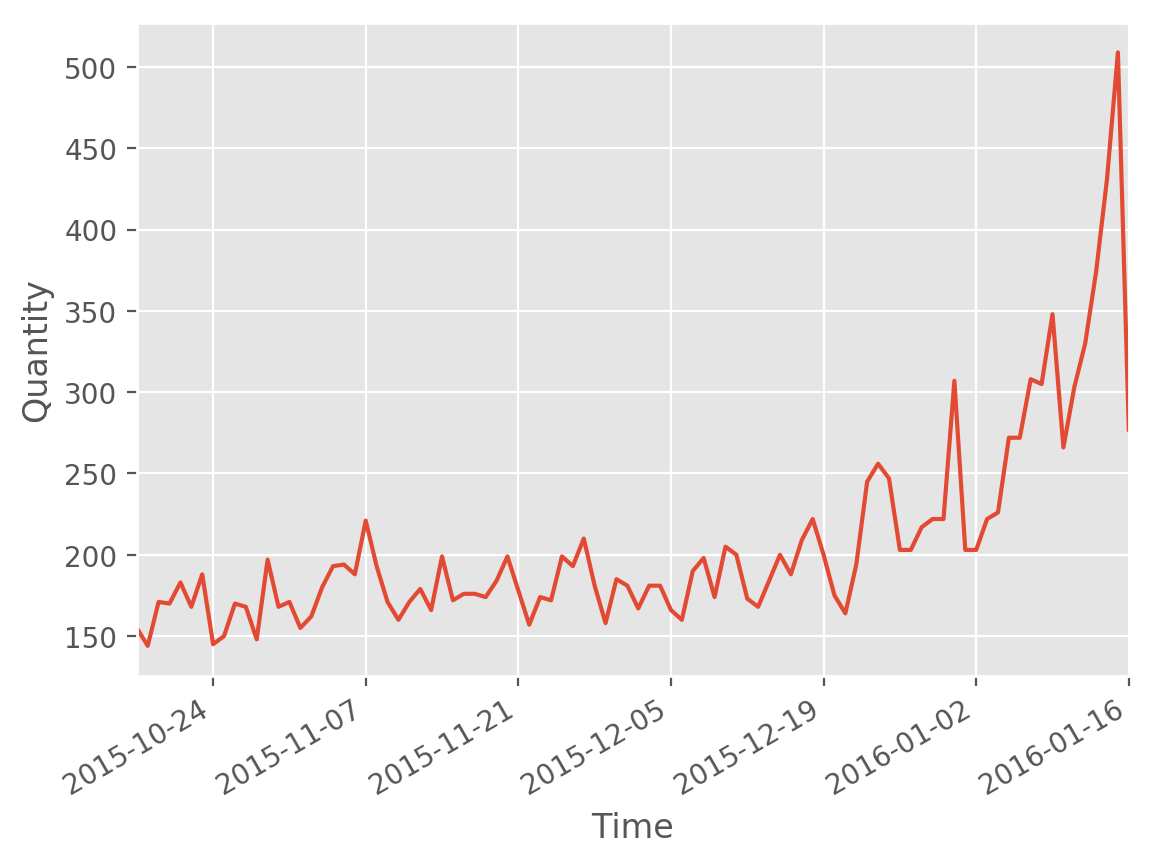
\includegraphics[width=\columnwidth]{quantity_time_graph}
  \caption{貼文數量對時間的關係圖}
  \label{f1}
  \end{figure}
  \end{center}
\end{minipage}
\quad
\begin{minipage}{0.43\textwidth}
  \begin{figure}[!htbp]
  \centering
  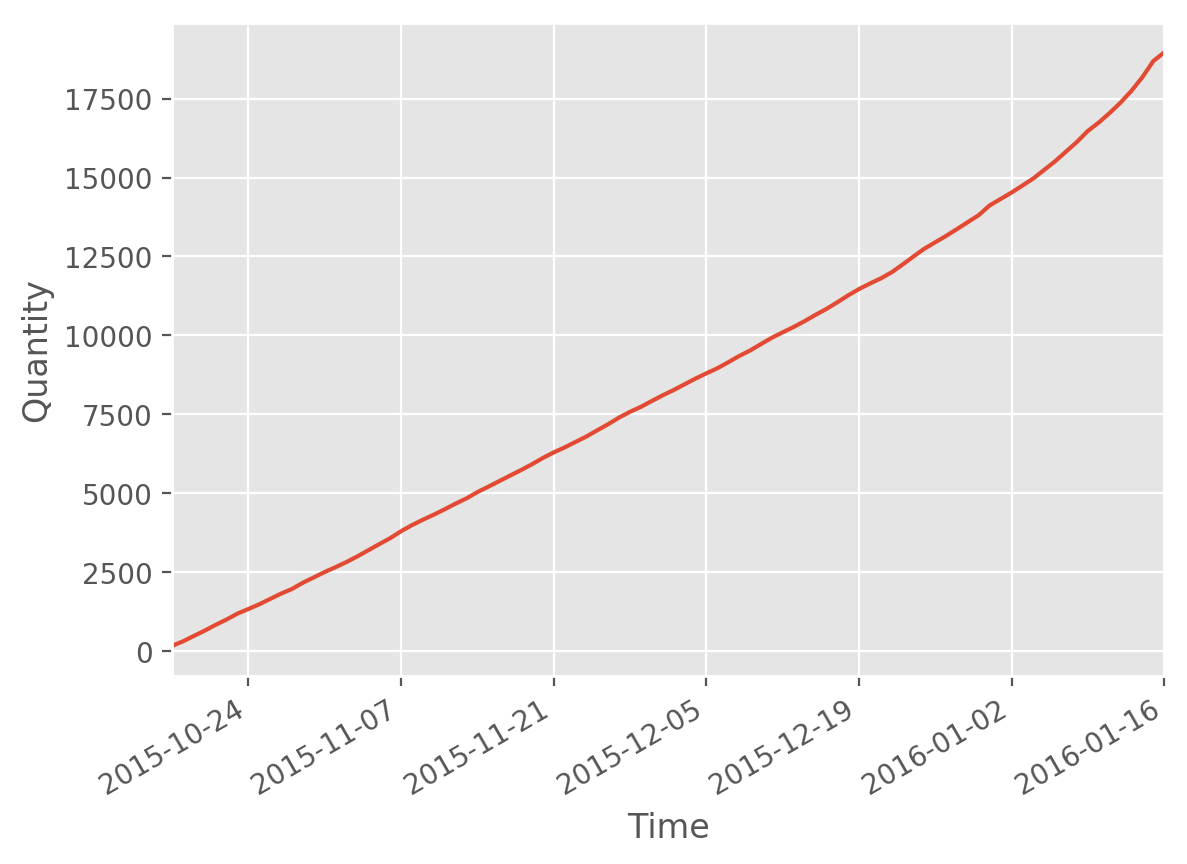
\includegraphics[width=\columnwidth]{quantity_time_cumulative_graph}
  \caption{累計貼文數量對時間的關係圖}
  \label{f2}
  \end{figure}
\end{minipage}
\end{center}
\end{block}
\end{minipage}

\begin{minipage}{0.30\textwidth}
\begin{block}{總體分佈(續)}
  \begin{table}[!htbp]
  \caption{各粉絲專頁的貼文數量(節錄)}
  \label{t1}
  \begin{tabular}{@{}L{12cm}C{5cm}C{5cm}@{}}
  \toprule
  粉絲專頁名稱 & 貼文數量 & 百分比 \\
  \midrule
  柯建銘 & 485 & 2.56\% \\
  Taiwan Fugue & 361 & 1.90\% \\
  台灣新力量/羅致政\dots & 337 & 1.78\% \\
  宋楚瑜找朋友 & 334 & 1.76\% \\
  反馬英九聯盟 & 330 & 1.74\% \\
  林昶佐 Freddy Lim & 320 & 1.69\% \\
  基進黨(基進側翼) & 319 & 1.68\% \\
  BillyPan 潘建志醫師 & 306 & 1.61\% \\
  宋楚瑜 & 301 & 1.59\% \\
  綠黨 & 297 & 1.57\% \\
  民主進步黨 & 293 & 1.54\% \\
  鄭永金後援會 & 282 & 1.49\% \\
  我是台灣人 (I am\dots & 281 & 1.48\% \\
  江啟臣服務讚 & 262 & 1.38\% \\
  \bottomrule
  \end{tabular}
  \end{table}
\end{block}
\end{minipage}
\quad
\begin{minipage}{0.68\textwidth}
\begin{block}{關鍵字擷取}
\begin{minipage}{0.34\textwidth}
  從表 \ref{t2} 我們可以看出各政黨/侯選人/意見領袖重視的議題。%
  例如,中國國民黨關注朱立倫、經濟、兩岸等事務,王金平關注國會、改革等事務,%
  綠黨關注勞工、環境等議題,而馬躍.比吼則關注原住民的文化和土地等等。%
  透過表 \ref{t3},我們可以發現人們關注的焦點皆圍繞在台灣、中國、國民黨上,唯有在 11 月 1 日至 11 月 8 日間,%
  由於舉行兩岸領導人會面,馬英九、馬習會也躍升為社群網站上的討論焦點。%
  表 \ref{t4} 告訴我們本次選舉人們最關心跟台灣和中國有關的議題,而國民黨也是人們討論的焦點。%
  值得一提的是,此次選舉的另一大黨,民主進步黨,並未出現在前十大關鍵字之中。%
\end{minipage}
\quad
\begin{minipage}{0.30\textwidth}
  \begin{table}[!htbp]
  \caption{依作者劃分(節錄)}
  \label{t2}
  \begin{tabular}{@{}L{8.5cm}ll@{}}
  \toprule
  粉絲專頁名稱 & \#1 & \#2 \\
  \midrule
  朱立倫 & 台灣 & 新 \\
  大安推范雲 & 范雲 & 台灣 \\
  王丹网站 Wa\dots & 中國 & 中 \\
  國民黨青年團 & 青年 & 台灣 \\
  呂欣潔 Jennif\dots & 政治 & 欣潔 \\
  管碧玲 (kuan\dots & 管媽 & 市長 \\
  段宜康 & 朱立倫 & 國民黨 \\
  鄉民實業坊 & 黑子 & 種 \\
  我是台灣人 (\dots & 台灣 & 綠黨 \\
  林智堅 & 新竹市 & 新竹 \\
  BillyPan 潘\dots & 醫師 & 台灣 \\
  蔡錦隆加油讚 & 蔡錦隆 & 錦隆 \\
  馬英九 & 臺灣 & 中 \\
  醫勞盟 & 醫師 & 醫療 \\
  \bottomrule
  \end{tabular}
  \end{table}
\end{minipage}
\quad
\begin{minipage}{0.29\textwidth}
  \begin{table}[!htbp]
  \caption{依時間劃分(節錄)}
  \label{t3}
  \begin{tabular}{@{}L{7.5cm}llllllllll@{}}
  \toprule
  時間區間 & \#1 & \#3 \\
  \midrule
  11/15 $\sim$ 11/22 & 台灣 & 政府 \\
  11/08 $\sim$ 11/15 & 台灣 & 中國 \\
  11/01 $\sim$ 11/08 & 台灣 & 中國 \\
  10/25 $\sim$ 11/01 & 台灣 & 國民黨 \\
  10/17 $\sim$ 10/25 & 台灣 & 新 \\
  \bottomrule
  \end{tabular}
  \end{table}
  \vspace{1em}
  \begin{table}[!htbp]
  \caption{合併所有貼文(節錄)}
  \label{t4}
  \begin{tabular}{@{}lll@{}}
  \toprule
  \#1 & \#3 & \#7 \\
  \midrule
  台灣  & 國民黨 & 中國  \\
  \bottomrule
  \end{tabular}
  \end{table}
\end{minipage}
\end{block}
\end{minipage}

\begin{minipage}{0.395\textwidth}
\begin{block}{這是一串中文}
圖 \ref{f1} 是貼文數量對時間的關係圖,橫軸為時間,以日為單位,縱軸為貼文數量,以篇為單位。%
圖 \ref{f2} 是累計貼文數量對時間的關係圖,橫軸為時間,以日為單位,縱軸為累計貼文數量,以篇為單位。%
從這兩張圖我們可以看出,隨著投票日的接近,各政黨/侯選人/意見領袖也愈來愈踴躍地在社群網站上發佈貼文。%
選舉前幾天的貼文數量更達到其餘時間的兩倍以上。%

    \begin{center}
      在這裡輸入文字。
    \end{center}

\end{block}
\end{minipage}
\quad
\begin{minipage}{0.585\textwidth}
\begin{block}{不知道要打什麼}
  \begin{center}
    在這裡輸入文字。
    \vspace*{8mm}
  \end{center}
  \begin{itemize}
    \item 在這裡輸入文字。
    \item 在這裡輸入文字。
    \item 在這裡輸入文字。
    \item 在這裡輸入文字。
    \item 在這裡輸入文字。
    \item 在這裡輸入文字。
  \end{itemize}
\end{block}
\end{minipage}

\begin{minipage}{0.64\textwidth}
\begin{block}{重要參考文獻}
  \nocite{*}
  \bibliographystyle{IEEEtran}
  \bibliography{citation}  
\end{block}
\end{minipage}
\quad
\begin{minipage}{0.34\textwidth}
\begin{alertblock}{\textbf{摘要}}
  \begin{itemize}
    \item 在這裡輸入文字。
    \item 在這裡輸入文字。
    \item 在這裡輸入文字。
  \end{itemize}
\end{alertblock}
\end{minipage}

\end{frame}
\end{CJK}
\end{document}
